\section{Measurements of $\phi_s$ and $\Delta\Gamma_s$}
\label{sec:phisdgs}

The $\phi_s$ weak phase and $B^0_s$ meson decay width difference can
be extracted by a time dependent full angular decay analysis of the 
$B^0_s \to J/\psi K^+ K^-$ decays. Such measurements have traditionally
used the subset of decays where the $K^+ K^-$ pair originates in the decay
of a $\phi$ meson, because its narrow width allows for an excellent background
rejection, but since the conference the first measurement which uses
the full $K^+ K^-$ mass spectrum~\cite{LHCbKKHighMass} has become available, and
more such measurements are expected in the future. The importance of
$\phi_s$ is that, in the absence of significant loop-diagram contributions
to $B^0_s \to J/\psi K^+ K^-$ decays (``penguin pollution''),
its value is precisely predicted~\cite{PHISSM} in the SM
\begin{equation}  
\phi_s = -0.036 \pm 0.002 \; ,
\end{equation}
and accurate experimental measurements of $\phi_s$ are therefore 
sensitive probes of the presence of BSM effects in the mixing and decay of $B^0_s$ mesons.

The results that the ATLAS and CMS Experiments obtained on their Run1
datasets using $B^0_s \to J/\psi \phi$ decays are:
\begin{eqnarray}
  \phi_s & = & -0.090 \pm 0.078 (\mbox{stat}) \pm 0.041 (\mbox{syst})\:[\mbox{rad}] \; , \\
  \Delta\Gamma_s & = & \phantom{-}0.085 \pm 0.011 (\mbox{stat}) \pm 0.007 (\mbox{syst})\:[\mbox{ps}^{-1}]  \; ,
\end{eqnarray}
for ATLAS \cite{atlas_phis_8TeV} and:
\begin{eqnarray}
  \phi_s & = & -0.075 \pm 0.097 (\mbox{stat}) \pm 0.031 (\mbox{syst})\:[\mbox{rad}]  \; , \\
  \Delta\Gamma_s & = & \phantom{-}0.095 \pm 0.013 (\mbox{stat}) \pm 0.007 (\mbox{syst})\:[\mbox{ps}^{-1}]  \; ,
\end{eqnarray}
for CMS \cite{cms_phis}. As can be seen in Fig.~\ref{phis_atlas_cms} both measurements are in
excellent agreement with the SM expectations.

\begin{figure}
  \begin{center}
    \begin{tabular}{c c}
      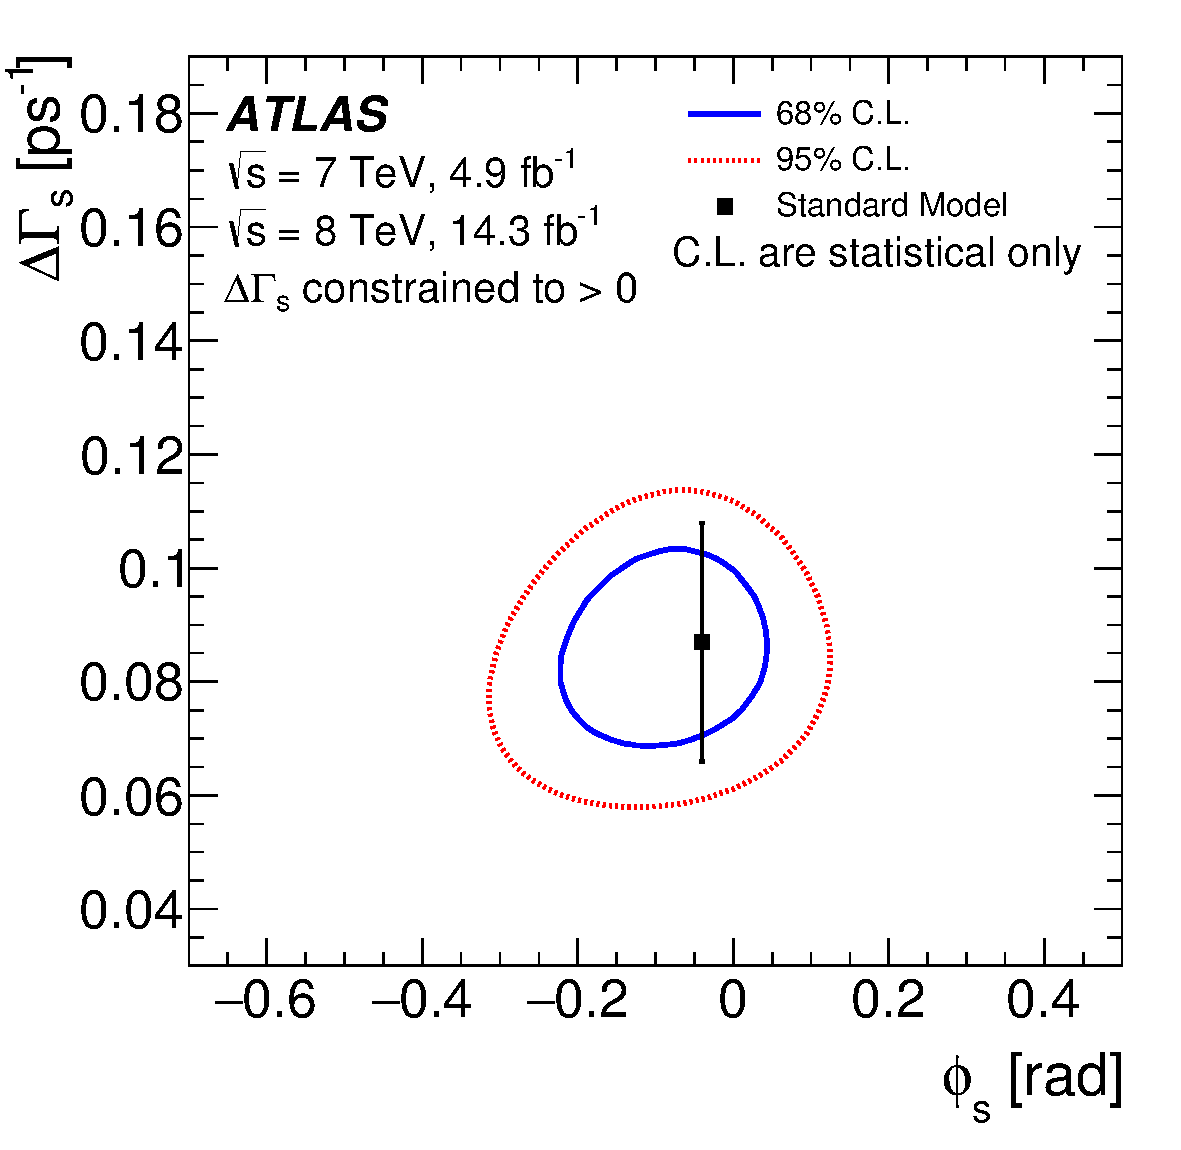
\includegraphics[height=5.5cm]{figs/atlas_phis_result.pdf} &
      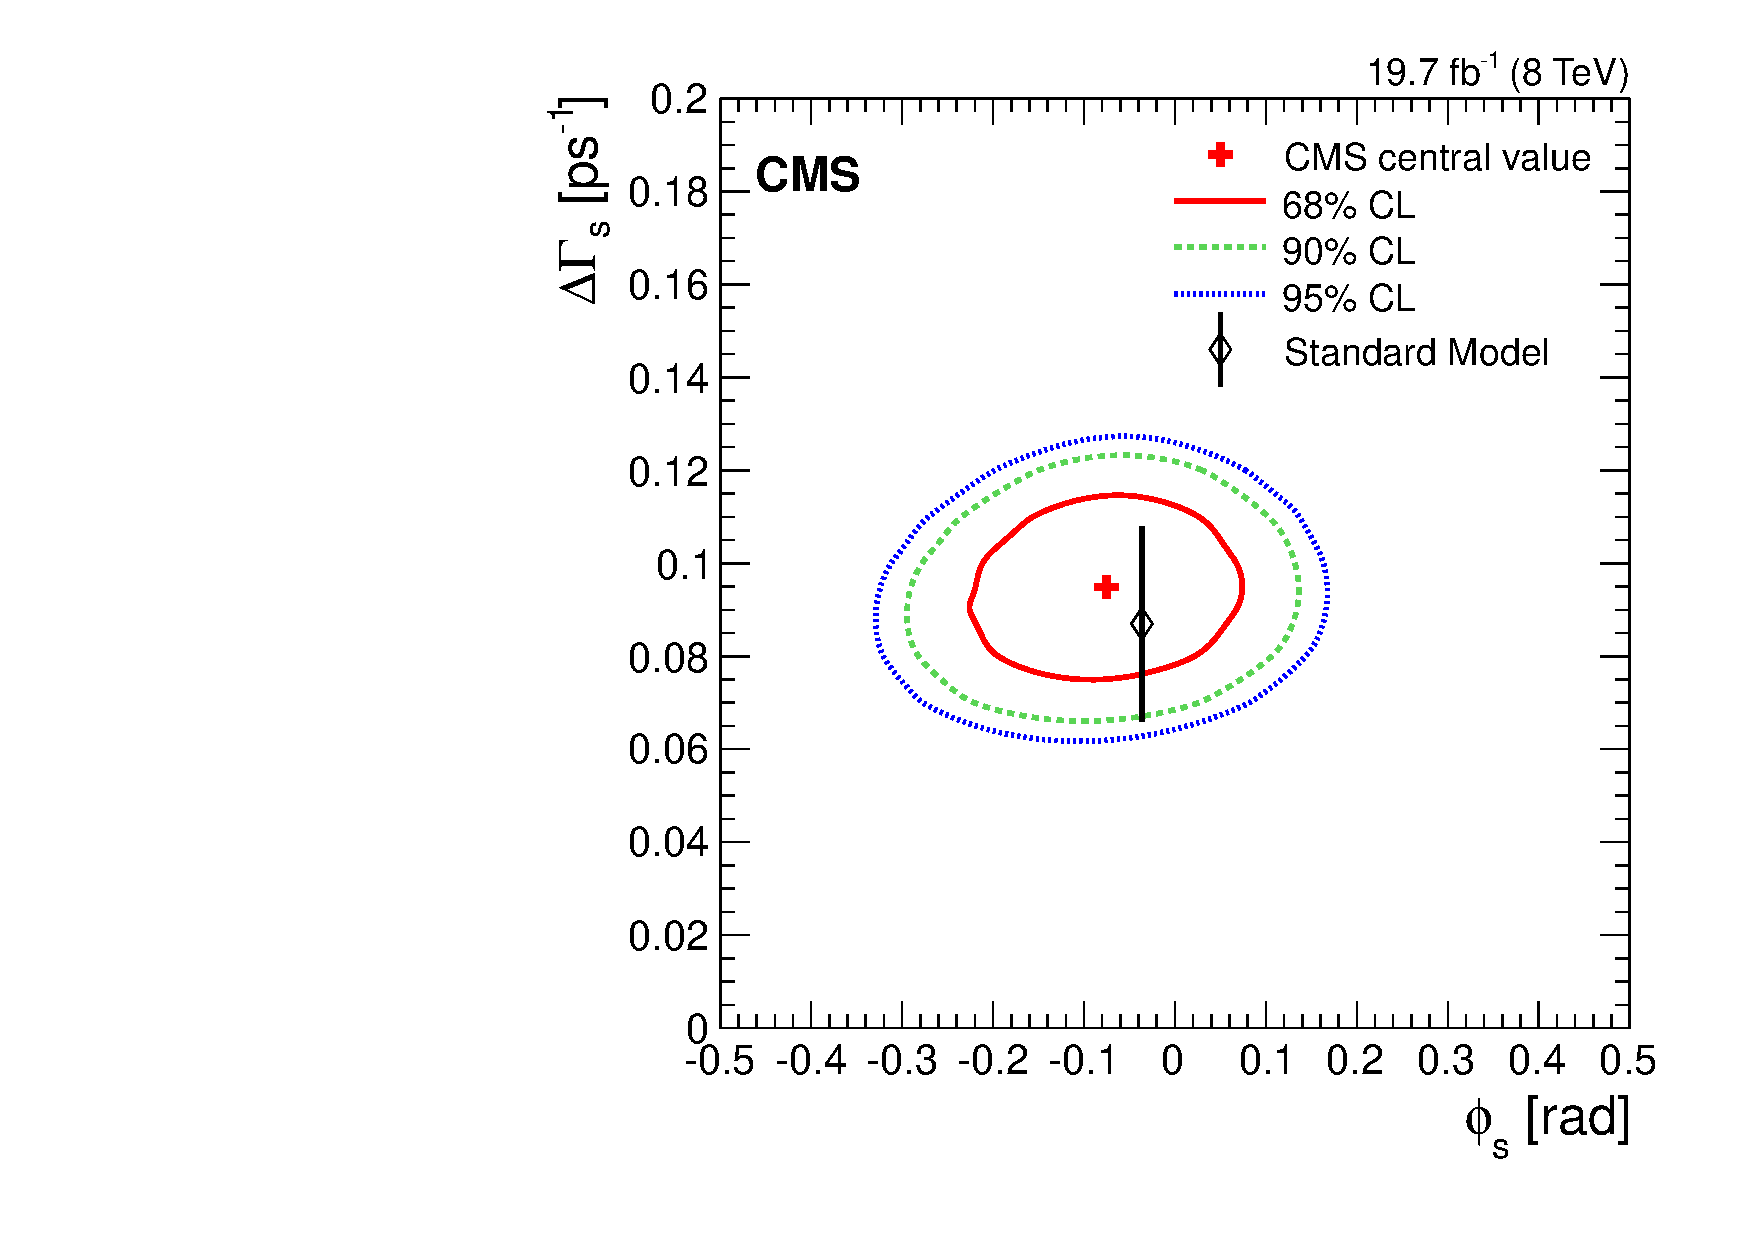
\includegraphics[height=5.5cm]{figs/cms_phis_result.pdf} 
    \end{tabular}
  \end{center}
  \vspace{-0.5cm}
  \caption{\label{phis_atlas_cms}Results on $\phi_s$ and $\Delta\Gamma_s$ from
  $B^0_s \to J/\psi \phi$ decays from (left) ATLAS~\cite{atlas_phis_8TeV} and (right) CMS~\cite{cms_phis}, reproduced from the respective citations.}
\end{figure}

The LHCb measurements of $\phi_s$ are covered in detail elsewhere in these proceedings~\cite{LHCBPHISPROC}.
LHCb uses not only $B^0_s \to J/\psi \phi$ but also $\Bs\to \jpsi\pi^+\pi^-$ decays,
where the $\pi^+\pi^-$ system is dominated by the $f_0(980)$ resonance and is greater than $97.7\%$ \CP-odd.
In this case no angular analysis is required, considerably simplifying the measurement
and providing important complementarity of systematic uncertainties.
The analysis of $B^0_s \to J/\psi \phi$ finds $\Delta\Gamma_s = 0.0805  \pm 0.0091         \pm  0.0032$~ps$^{-1}$,
where the first uncertainty is statistical and the second systematic. 
A combination of $B^0_s \to J/\psi \phi$ and $\Bs\to \jpsi\pi^+\pi^-$ gives $\phis = -0.010  \pm  0.039$~rad, which is the most 
precise single-experiment determination of this quantity.
LHCb has also measured $\phi_s$ using $\Bs\to \psi(2S)\phi$ decays, obtaining
$0.23^{+0.29}_{-0.28} \pm 0.02$ rad.

While $B^0_s \to J/\psi K^+ K^-$ is expected to be dominated by the tree-level diagram,
as the experimental precision on $\phi_s$ improves it will become increasingly important
to account for residual penguin pollution in order to correctly interpret any agreement,
or otherwise, with the theoretical prediction. The size of such effects can be controlled
using a combination of $B^0_s \to J/\psi K^{*0}$ and $B^0 \to J/\psi \rho$ decays,
which are related by U-spin symmetry and in the limit of zero non-factorizable SU(3)
breaking are sensitive to the same, universal, penguin amplitudes and phases.
LHCb has performed measurements of both modes~\cite{LHCb-PAPER-2015-034,LHCb-PAPER-2014-058} and
measures essentially zero penguin pollution to $\phi_s$ with a precision of around 15~mrad
in all three polarization-dependent phases. The LHCb measurement is statistics limited
and penguin pollution to $\phi_s$ should therefore
remain under control as the experimental precision approaches the SM value.

In addition to comparisons with the SM prediction, such tree-dominated measurements of $\phi_s$ can also be compared with the measurement
of the related quantity $\phi_s^{ss\overline{s}}$ in the loop-dominated decays $\Bs \to \phi\phi$ and $\Bs\to \Kp\pi^-\Kp\pi^-$.
In the absence of BSM physics effects, this quantity is expected to be very close to zero.
LHCb has measured~\cite{LHCb-PAPER-2014-026} $\phi_s^{ss\overline{s}} = -0.17 \pm 0.15 \pm 0.03$ rad using
$\Bs\to \phi\phi$, in excellent agreement with the SM prediction. The measurement,
which uses $\Bs\to \Kp\pi^-\Kp\pi^-$, is ongoing; it is considerably more challenging and
requires a two-dimensional Dalitz analysis to account
for the interfering intermediate resonances. 

LHCb has also measured~\cite{LHCb:2017ood} the time-dependent $CP$ violation in $B^0 \to \pi^+ \pi^-$ and $B^0_s \to K^+ K^-$ decays.
These can be interpreted\footnote{In the absence of information about $B^0_s \to K^+ K^-$, measurements of time-dependent $CP$ violation in
$B^0 \to \pi^+ \pi^-$ have traditionally~\cite{HFAG} been combined with other two-body $B^0$ decays in an isospin analysis to obtain a measurement of $\alpha$.}
in a combined U-spin analysis~\cite{Fleischer:1999pa} as either measurements of $\gamma$ or $\phi_s$.
Because the combined U-spin analysis is much less sensitive
to U-spin breaking~\cite{LHCb-PAPER-2014-045} when interpreted as a measurement of $\phi_s$, this is therefore the currently preferred way
to interpret the measurements of these $CP$ observables.

$CP$ violation in $B^0 \to \pi^+ \pi^-$ has been measured previously by BaBar~\cite{Lees:2012mma} and Belle~\cite{Adachi:2013mae},
while the measurement of $B^0_s \to K^+ K^-$ is unique to LHCb. Using a two-dimensional fit to the mass and decay-time
of the neutral $B$ mesons, LHCb observes $CP$ violation in the interference of mixing and decay of $B^0_s$ mesons for the first time, 
and finds
\begin{eqnarray}
C_{\pi\pi}      &=& -0.24 \pm 0.07 \pm 0.01,\phantom{space}
S_{\pi\pi}      = -0.68 \pm 0.06 \pm 0.01,\phantom{space}
\\
C_{KK}      &=& \phantom{+}0.24 \pm 0.06 \pm 0.02,\phantom{space}
S_{KK}      = \phantom{+}0.22 \pm 0.06 \pm 0.02,\phantom{space}
\\
A^{\Delta}_{KK}      &=& -0.75 \pm 0.07 \pm 0.11,\phantom{space}
\end{eqnarray}
where the first uncertainty is statistical and the second systematic. It can be seen that the (co)sinusoidal $C$ and $S$ parameters have
negligible systematic uncertainties, while the hyperbolic $A^{\Delta}_{KK}$, which is sensitive to differences in the distributions
of $B^0_s$ and $\bar{B^0_s}$ induced by $\Delta\Gamma_s$ at high decay-times, is much more sensitive to experimental effects.
This is the most precise single-experiment
determination of $S_{\pi\pi}$, and significantly improves the world-average of this parameter as shown in Fig.~\ref{b2pipiwahfag}.
A combined interpretation in terms of $\phi_s$ is not available at the time of writing but is expected to be performed
in the future, and both LHCb and Belle-II are expected to improve our knowledge of the $CP$ observables in the future. 
The measurement of $A^{\Delta}_{KK}$ is a world first, allowing for a twofold reduction in the ambiguity of the $\phi_s$ determination
and can also be interpreted as a measurement of $\Delta\Gamma_s$.

\begin{figure}
  \begin{center}
    \begin{tabular}{c c}
      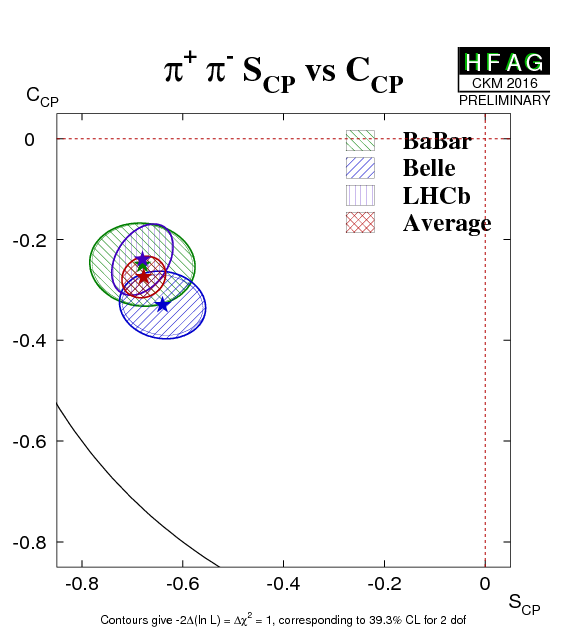
\includegraphics[height=7.5cm]{figs/pi+pi-S_CPvsC_CP.png} &
    \end{tabular}
  \end{center}
  \vspace{-0.5cm}
  \caption{\label{b2pipiwahfag}World average of time-dependent $CP$ observables in $B^0 \to \pi^+ \pi^-$, reproduced from HFAG~\cite{HFAG}.}
\end{figure}
